\begin{frame}{Introduction}{State-of-affairs and motivation}
	\begin{itemize}
		\item Energy demand is still rising
		\item Wind energy is a part of solution to lower CO2 emissions
		\item LCOE higher in offshore wind turbines but there are advantages
		\item Shallow-water depth sites (<50 m) will eventually exhaust
		\item Floating turbines are in prototype stage but maturing
		\item In recent news: "\textit{Portugal to auction 3-4 GW of floating offshore wind farms in summer}" (\href{https://www.reuters.com/business/energy/portugal-auction-3-4-gw-floating-offshore-wind-farms-summer-2022-03-16/}{Article link})
	\end{itemize}\bigskip
\end{frame}

%%%%%%%%%%%%%%%%%%

\begin{frame}{Introduction}{Wind turbine components}
	Relevant components:
	\begin{itemize}
		\item Rotor, blades, pitch system
		\item Tower
		\item Generator
	\end{itemize}
	\begin{figure}[ht]
		\centering
		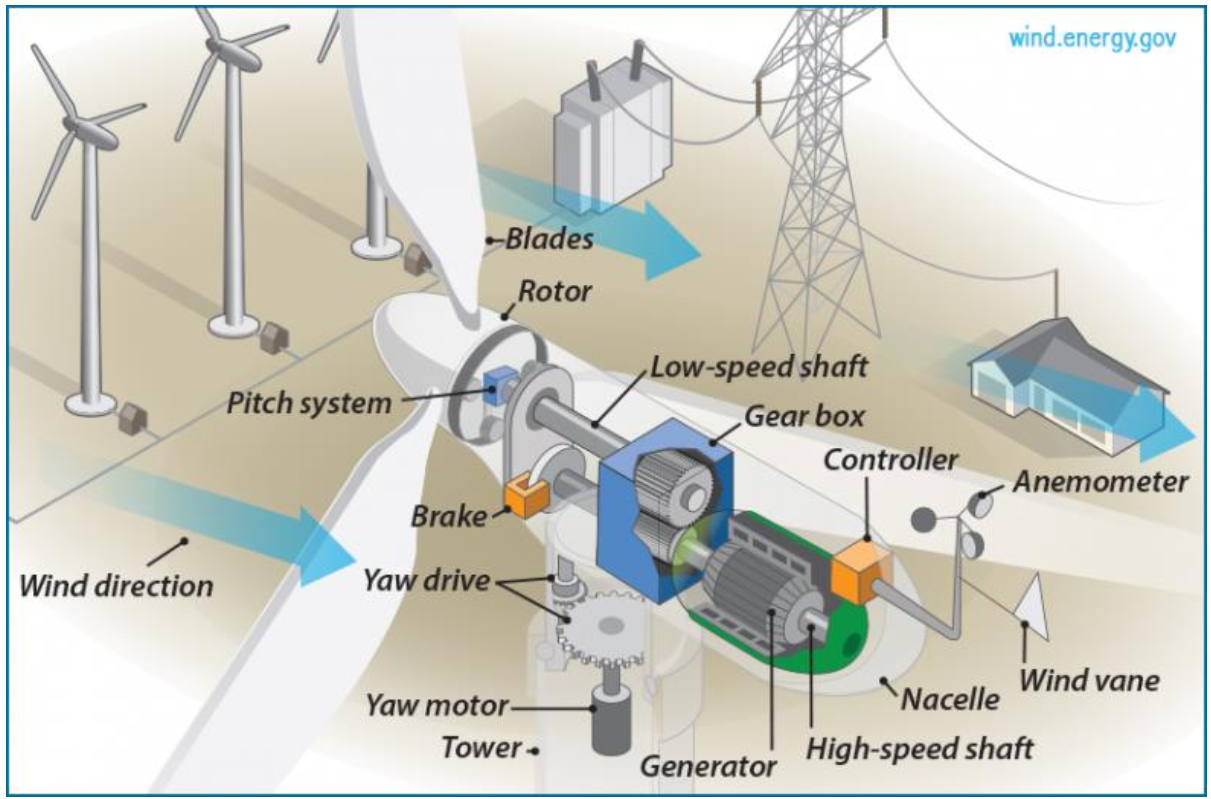
\includegraphics[width=0.7\linewidth]{../Graphics/WtComponents.png}
		\label{fig:wt_components}
	\end{figure}

\end{frame}

%%%%%%%%%%%%%%%%

\begin{frame}{Introduction}{Floating offshore wind turbines}
	\begin{itemize}
		\item Characterized by static stability which counteracts overturning moment
		\item Restoring force is sum of: Buoyancy, ballast and mooring line forces
	\end{itemize}
	Four main foundation concepts:
	\begin{figure}[ht]
		\centering
		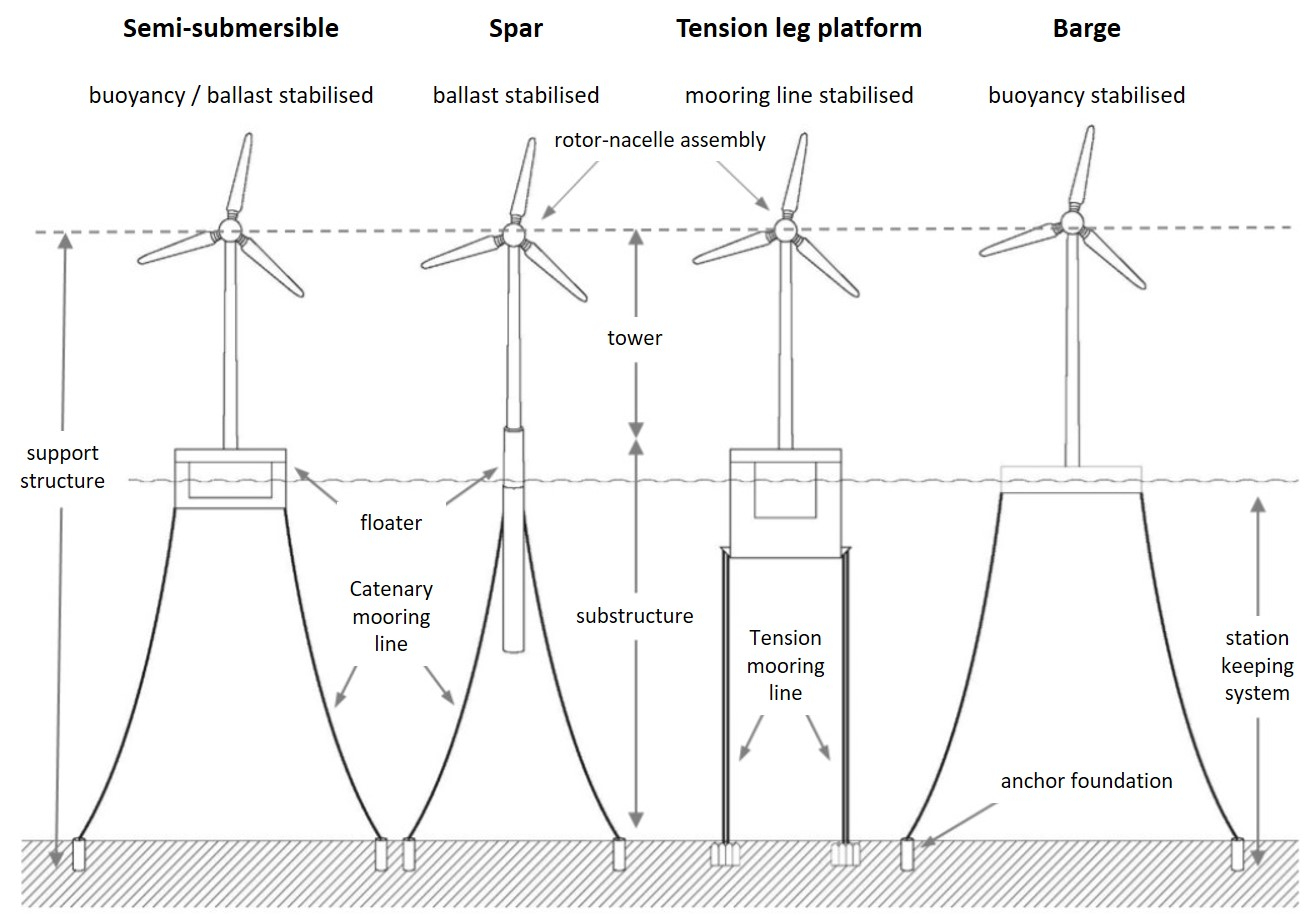
\includegraphics[width=.8\linewidth]{../Graphics/FloatingFoundationConcepts.jpg}
		\label{fig:floating_concepts}
	\end{figure}
\end{frame}

%%%%%%%%%%%%%%%%

\begin{frame}{Introduction}{Floating offshore wind turbines}
	\begin{columns}
		\begin{column}{.49\textwidth}
			\begin{itemize}
				\item Subjected to additional loads
				\item Experiences higher strain due to extra degrees of freedom $ \rightarrow $ higher LCOE
				\item The negative damping problem
				\item Load reduction = LCOE reduction = better feasibility
			\end{itemize}
		\end{column}
		
		\begin{column}{.49\textwidth}
			The 6 additional degrees of freedom of a FOWT:
			\begin{figure}[ht]
				\centering
				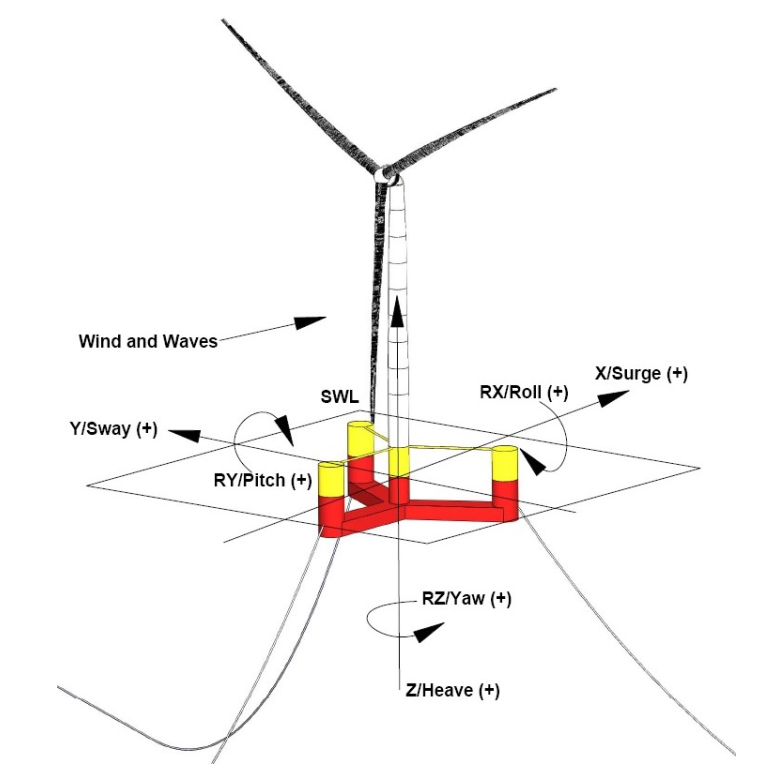
\includegraphics[width=1\linewidth]{../Graphics/FOWTcoordinates.png}
				\label{fig:fowt_coordinates}
			\end{figure}	
		\end{column}
	\end{columns}
\end{frame}


%%%%%%%%%%%%%%%%%%
%\begin{frame}{Big header}{Smaller header}
%	\textbf{Some text}
%	\begin{itemize}
%		\item Item
%	\end{itemize}
%\end{frame}
%


%%%%%%%%%%%%%%%%%%

%\begin{frame}{Big header}{Smaller header}
	%\begin{columns}
	%	\begin{column}{.49\textwidth}
	%		
	%	\end{column}
	%	
	%	\begin{column}{.49\textwidth}
	%	
	%	\end{column}
	%\end{columns}
%\end{frame}